% ---------------------------------------------------------------------
% 2.3 Potenciales relacionados con eventos y componente P300
% ---------------------------------------------------------------------
\section[POTENCIALES RELACIONADOS CON EVENTOS Y COMPONENTE P300]{Potenciales relacionados con
eventos y componente P300}
\label{sec:erp}

\subsection{Potenciales relacionados con eventos}

La mayor parte de la actividad del EEG se presenta de manera espontánea. En cambio, los potenciales relacionados con
eventos (ERP, por sus siglas en inglés) son variaciones del voltaje que aparecen ligadas en el tiempo
a un evento específico. Este evento puede ser un estímulo sensorial, una respuesta motora o una
operación cognitiva, como reconocer un estímulo \cite{kropotov2009}. En el cuero cabelludo, un ERP
se registra como una serie de ondas positivas y negativas llamadas componentes. Cada componente se
nombra con la letra P o N según su polaridad, seguida de un número que indica su latencia
aproximada en milisegundos o su posición en la secuencia \cite{luck2014}. La
Tabla~\ref{tab:componentes} describe las componentes que aparecen con mayor frecuencia en
paradigmas de estimulación visual, y la Figura~\ref{fig:erp} muestra la forma de onda típica de un
ERP ante un estímulo objetivo y ante uno no objetivo, en la que la P300 solo aparece en el primero.

\begin{table}[htbp]
\centering
\caption{Principales componentes de los ERP en paradigmas visuales}
\label{tab:componentes}
\small
\begin{tabularx}{\textwidth}{L{2.1cm}L{2.1cm}L{2.0cm}Y}
\toprule
\textbf{Componente} & \textbf{Latencia} & \textbf{Polaridad} & \textbf{Proceso asociado} \\
\midrule
N100 (N1) & 100--200 ms & Negativa & Procesamiento sensorial y orientación de la atención hacia el estímulo. \\
P200 (P2) & 150--250 ms & Positiva & Evaluación de las características físicas del estímulo. \\
N200 (N2) & 200--350 ms & Negativa & Detección de desajuste entre el estímulo y lo esperado, y clasificación del estímulo. \\
P300 (P3) & 250--500 ms & Positiva & Actualización del contexto en la memoria de trabajo ante estímulos relevantes o poco frecuentes. \\
\bottomrule
\end{tabularx}
\par\smallskip{\footnotesize Elaboración propia con información de \cite{luck2014,kropotov2009,polich2007}.}
\end{table}

\begin{figure}[htbp]
\centering
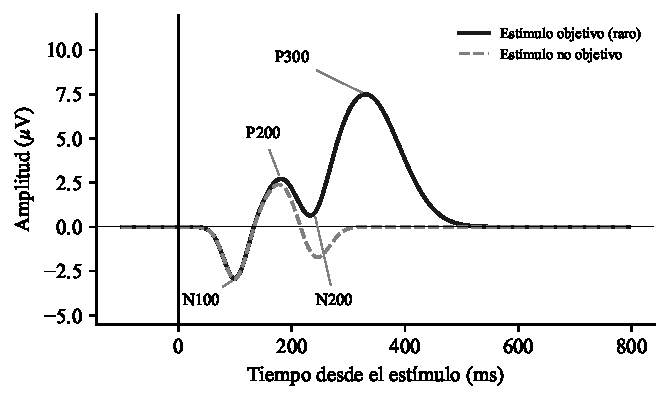
\includegraphics[width=0.75\textwidth]{02-marco-referencial/erp_componentes.pdf}
\caption{Forma de onda ilustrativa de un ERP ante un estímulo objetivo y uno no objetivo, con las
latencias de la Tabla~\ref{tab:componentes}. Elaboración propia con base en
\cite{luck2014,polich2007}.}
\label{fig:erp}
\end{figure}

\subsection{Promediado coherente}

El principal problema para observar un ERP es que su amplitud, de unos cuantos microvolts, es
considerablemente menor que la de la actividad de fondo del EEG, que para estos fines se comporta
como ruido. La forma clásica de resolverlo consiste en presentar el mismo estímulo repetidas veces,
extraer los segmentos de señal sincronizados con cada presentación y promediarlos
\cite{tong2009}. Si cada ensayo $x_i(n)$ se modela como la suma de una respuesta $s(n)$ que se
repite de forma idéntica y de un ruido $r_i(n)$ de media cero y varianza $\sigma^2$, independiente
entre ensayos, el promedio de $N$ ensayos queda como
\begin{equation}
\bar{x}(n) = \frac{1}{N}\sum_{i=1}^{N} x_i(n) = s(n) + \frac{1}{N}\sum_{i=1}^{N} r_i(n),
\label{eq:promediado}
\end{equation}
donde la desviación estándar del ruido residual se reduce a $\sigma/\sqrt{N}$, de modo que la
relación señal-ruido mejora en proporción a la raíz cuadrada del número de ensayos
\cite{luck2014}. Esta relación explica por qué el P300 Speller necesita repetir varias veces la
intensificación de cada fila y columna, y por qué reducir dichas repeticiones, objetivo de este
trabajo, compromete directamente la confiabilidad de la detección.

\subsection{La componente P300}

La componente P300 fue descrita por primera vez en 1965 por Sutton et al., quienes observaron que
los estímulos cuya ocurrencia era incierta para el sujeto evocaban una onda positiva de gran
amplitud alrededor de 300~ms después de su presentación \cite{sutton1965}. Años más tarde, Squires,
Squires y Hillyard distinguieron dos variantes de esta onda \cite{squires1975}, de las cuales el
P300 Speller aprovecha la P3b, que se registra en la región parietal y aparece ante estímulos
relevantes para la tarea, pues su aparición depende de que el usuario atienda deliberadamente al
carácter que desea seleccionar \cite{polich2007}.

La P300 se describe principalmente con dos medidas. La amplitud es la diferencia entre el voltaje
de la línea base previa al estímulo y el pico positivo más alto, que se busca típicamente entre 250
y 500~ms. La latencia es el tiempo que pasa desde el inicio del estímulo hasta ese pico
\cite{polich2007}. En los electrodos de la línea media, la amplitud aumenta de las regiones
frontales hacia las parietales y alcanza su máximo en Pz \cite{picton1992}. La amplitud es mayor
cuando el estímulo objetivo es menos probable y más relevante para la tarea. En cambio, disminuye
con la fatiga, la habituación y los intervalos cortos entre estímulos
\cite{polich2007,picton1992}.

\subsection{Paradigma del evento raro}

El procedimiento experimental más utilizado para provocar la P300 es el paradigma del evento raro,
conocido en inglés como \textit{oddball}. En él se presenta al sujeto una secuencia de estímulos de
dos categorías, una de las cuales aparece con mucha menor frecuencia que la otra, y se le pide que
atienda o cuente únicamente los estímulos de la categoría poco frecuente
\cite{farwell1988,polich2007}. Los estímulos raros, que en el contexto de una BCI corresponden al
objetivo elegido por el usuario, producen una P300 cuya amplitud es inversamente proporcional a su
probabilidad de aparición \cite{farwell1988}. La Figura~\ref{fig:oddball} representa una secuencia
típica de este paradigma.

\begin{figure}[htbp]
\centering
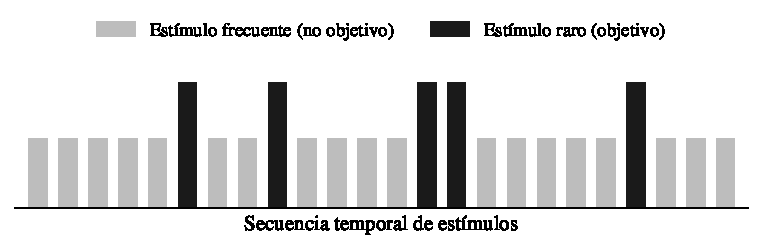
\includegraphics[width=0.9\textwidth]{02-marco-referencial/oddball.pdf}
\caption{Secuencia de estímulos en el paradigma del evento raro (\textit{oddball}). Elaboración
propia.}
\label{fig:oddball}
\end{figure}
